
\documentclass[a4paper,12pt]{article}

\usepackage[style=chicago-authordate]{biblatex}
\addbibresource{../bibfile.bib}

\usepackage[brazil]{babel}
\usepackage{amsmath}
\usepackage{geometry}
\geometry{a4paper, top=2.5cm, bottom=2.0cm, left=2.5cm, right=2.5cm} % Margens ajustadas
\usepackage{multirow, booktabs}
\usepackage{graphicx}
\usepackage{setspace}
\usepackage{float}
\usepackage{fancyhdr}
\usepackage{gensymb}
\usepackage{hyperref}
\usepackage{listings}
\usepackage{xcolor}
\usepackage{microtype}

\lstset{
    language=Octave,
    frame=single,
    numbers=left,
    numberstyle=\tiny,
    stepnumber=1,
    numbersep=5pt,
    backgroundcolor=\color{gray!10},
    showspaces=false,
    showstringspaces=false,
    showtabs=false,
    tabsize=4,
    captionpos=b,
    breaklines=true,
    breakatwhitespace=false,
    title=\lstname,
    basicstyle=\ttfamily,
    keywordstyle=\color{blue},
    commentstyle=\color{green!50!black},
    stringstyle=\color{red},
}

\pagestyle{fancy}
\fancyhf{}
\lhead{\footnotesize Cefet-MG: L07CSD - Solução da lista de exercícios VII}
\cfoot{\footnotesize \thepage}

\setlength{\footskip}{0.8cm} % Espaço entre o texto e o rodapé
\setlength{\headheight}{13.6pt} % Altura do cabeçalho

\setlength{\parindent}{0in}

\renewcommand{\arraystretch}{1.5} % Ajusta o espaçamento entre as linhas do array


\begin{document}

%%%%%%%%%%%%%%%%%%%%%%%%%%%%%%%%%%%%%%%%%%%%%%%%
% Seção de Título
%%%%%%%%%%%%%%%%%%%%%%%%%%%%%%%%%%%%%%%%%%%%%%%%

    \thispagestyle{empty} % Desativa cabeçalho na primeira página

    \begin{tabular}{p{15.5cm}}
    {\large \textbf{Controle de Sistemas Dinâmicos} } \\
    Centro Federal de Educação Tecnológica de Minas Gerais \\
    02 de dezembro de 2024 \\ Campus Timóteo \\
    \hline
    \\
    \end{tabular}

    \vspace*{0.3cm}

    \begin{center}
    {\Large \textbf{Resolução da lista de exercícios VII}}
        \vspace{2mm}

        {\textbf{Eliel Vitor Almeida \\ João Pedro Ferreira Duarte \\ Marcos Vinícius de Oliveira Silva }}
    \end{center}

    \vspace{0.4cm}

%%%%%%%%%%%%%%%%%%%%%%%%%%%%%%%%%%%%%%%%%%%%%%%%
% Corpo do Documento
%%%%%%%%%%%%%%%%%%%%%%%%%%%%%%%%%%%%%%%%%%%%%%%%

    Em sequência, estão os comandos e resoluções das questões da avaliação.
    Há também referências para quaisquer figuras e/ou ilustrações usadas durante o desenvolvimento do presente texto em
    espaço reservado ao fim da resolução das questões.
    \begin{enumerate}
        \item Crie as seguintes funções de transferência na forma polinomial:
        \[
            \begin{array}{ccc}
                \frac{3}{2s + 1} & \frac{3}{2s - 1} & \frac{5}{(s + 2) \cdot (s + 5)} \\
                \frac{5}{(s - 2) \cdot (s - 5)} & \frac{5}{s^2 + 2s + 5} & \frac{5}{s^2 - 2s + 5} \\
                \frac{5}{s^2 + 16} & \frac{5}{s^2 - 16} & \frac{5}{s^2 + 6s + 9} \\
            \end{array}
        \]

        \begin{enumerate}
            \item Calcule os pólos de cada função de transferência.
            \item Plote a resposta ao degrau de cada função de transferência. Use a função \texttt{step}.
            \item Descreva o comportamento de cada resposta obtida, fale sobre a estabilidade do sistema e relacione este comportamento aos pólos. Comente e conclua.
        \end{enumerate}
        Em resposta aos itens anteriores:
        \vspace{0.5cm}
        \begin{lstlisting}
pkg load control;

numerador_A = 3;
denominador_A = [2, 1];

numerador_B = 3;
denominador_B = [2, -1];

numerador_C = 5;
denominador_C = [-2,-5];

numerador_D = 5;
denominador_D = [2,5];

numerador_E = 5;
denominador_E = [1,2,5];

numerador_F = 5;
denominador_F = [1,-2,5];

numerador_G = 5;
denominador_G = [1,0,16];

numerador_H = 5;
denominador_H = [1,0,-16];

numerador_I = 5;
denominador_I = [1,6,9];
% Calcular os polos (raizes do denominador)
poles_A = roots(denominador_A);
poles_B = roots(denominador_B);
poles_C = roots(denominador_C);
poles_D = roots(denominador_D);
poles_E = roots(denominador_E);
poles_F = roots(denominador_F);
poles_G = roots(denominador_G);
poles_H = roots(denominador_H);
poles_I = roots(denominador_I);

% Exibir os polos
disp('Polos de A:');
disp(poles_A);

disp('Polos de B:');
disp(poles_B);

disp('Polos de C:');
disp(poles_C);

disp('Polos de D:');
disp(poles_D);

disp('Polos de E:');
disp(poles_E);

disp('Polos de F:');
disp(poles_F);

disp('Polos de G:');
disp(poles_G);

disp('Polos de H:');
disp(poles_H);

disp('Polos de I:');
disp(poles_I);

%Plotar no grafico

plot_A = tf(numerador_A,denominador_A);
step(plot_A,10);

plot_B = tf(numerador_B,denominador_B);
step(plot_B,10);

plot_C = tf(numerador_C,denominador_C);
step(plot_C,10);

plot_D = tf(numerador_D,denominador_D);
step(plot_D,10);

plot_E = tf(numerador_E,denominador_E);
step(plot_E,10);

plot_F = tf(numerador_F,denominador_F);
step(plot_F,10);

plot_G = tf(numerador_G,denominador_G);
step(plot_G,10);

plot_H = tf(numerador_H,denominador_H);
step(plot_H,10);

plot_I = tf(numerador_I,denominador_I);
step(plot_I,10);
        \end{lstlisting}
        Sobre os gráficos gerados pelas funções acima com o uso da função \texttt{step}, temos então \ref{fig1a}, \ref{fig1b}, \ref{fig1c}, \ref{fig1d}
        , \ref{fig1e}, \ref{fig1f}, \ref{fig1g}, \ref{fig1h} e \ref{fig1i} como figuras que representam estes gráficos.


        Em função das caracteríisticas já estudadas, conseguimos dizer que a presença de pólos reais no lado positivo do plano cartesiano,
        faz com que o sistema se torne instável, de forma que essa é uma característica comum nestes gráficos que damos como instáveis a seguir.
        %

        Verificamos como funções com respostas estáveis, \ref{fig1c}, \ref{fig1d}, \ref{fig1e} e \ref{fig1i}. Agora como instáveis, temos então
        \ref{fig1a}, \ref{fig1b}, \ref{fig1f}, \ref{fig1g} e \ref{fig1h}.

        \item Sejam os sistemas representados pelas seguintes funções:
        \[
            \begin{array}{cc}
                G_1 = \frac{1}{2s + 1}, & G_2 = \frac{1}{s^2 + 0.5s + 1}
            \end{array}
        \]
        \begin{enumerate}
            \item Verifique como tais sistemas respondem às seguintes entradas:
            \begin{enumerate}
                \item Rampa.
                \item Impulso.
                \\
                Plote o gráfico de cada uma das funções.
            \end{enumerate}
            Sobre o código de determinada implementação:
            \begin{lstlisting}
pkg load control;
pkg load symbolic;

syms s;

%2a
figure;
clf;
s = tf('s');
g = (1/(2*s +1))*(1/s);
step(g);
title ("Funcao step com a FT rampa 2a");

figure;
clf;
s = tf('s');
g = (1/(2*s +1))*(1/s);
impulse(g);
title ("Funcao impulse com a FT rampa 2a");

%2b
figure;
clf;
s = tf('s');
g = (1/(s^2 +0.5*s + 1))*(1/s);
step(g);
title ("Funcao step com a FT rampa 2b");

figure;
clf;
s = tf('s');
g = (1/(s^2 +0.5*s + 1))*(1/s);
impulse(g);
title ("Funcao impulse com a FT rampa 2b");
            \end{lstlisting}
            Os gráficos feitos em resposta ao código gerado, podem ser consultados abaixo, em \ref{fig2aStep}, \ref{fig2aImpulse}, \ref{fig2bStep} e
            \ref{fig2bImpulse}:
        \end{enumerate}
        \item Considere o sistema com realimentação descrito na figura anexa à atividade:
        \begin{enumerate}
            \item Calcule a função de transferência em malha fechada usando as funções \texttt{series} e \texttt{feedback}.
            \begin{lstlisting}
pkg load control;

sys1 = tf([1], [1, 1]);
sys2 = tf([1, 2], [1, 3]);

sysSeries = series(sys1, sys2);

sysFeedback = feedback(sys1, sys2);

disp('Sistema em serie:');
display(sysSeries);

disp('Sistema em malha fechada (feedback):');
display(sysFeedback);
            \end{lstlisting}
            Em resposta ao item, as seguintes funções de transferência foram retornadas:
            \begin{array}{cc}
                y_1 = \frac{s + 2}{s^2 + 4s + 3}, & y_2 = \frac{s + 3}{s^2 + 5s + 5}
            \end{array}
            \item  \label{3b} Obtenha a resposta ao degrau unitário do sistema em malha fechada com a função \texttt{step} e verifique que o valor final
            da saída é $\frac{2}{5}$.
            \begin{lstlisting}
pkg load control;

sys1 = tf([1], [1, 1]);
sys2 = tf([1, 2], [1, 3]);

sysSeries = series(sys1, sys2);

sysFeedback = feedback(sysSeries, 1);

disp('Sistema em série:');
display(sysSeries);

disp('Sistema em malha fechada (feedback):');
display(sysFeedback);

[num, den] = tfdata(sysFeedback, 'vetor');
valorFinal = dcgain(sysFeedback);

disp(['Valor final da saida: ', num2str(valorFinal)]);
            \end{lstlisting}
            Com valor de saída de \ref{3b} igual à $0.4$ ou $\frac{2}{5}$.
        \end{enumerate}

        \item Um sistema possui a seguinte função de transferência:
        \begin{equation}
            \frac{X(s)}{R(s)} = \frac{\frac{20}{z} \cdot (s + z)}{s^2 + 3s + 20}
        \end{equation}
        \begin{enumerate}
            \item Obtenha a resposta ao degrau unitário do sistema para o parâmetro \(z = 5\), \(z = 10\), e \(z = 15\).
            \item Plote as 3 curvas no mesmo gráfico. Compare, comente e conclua.
        \end{enumerate}
    \end{enumerate}

    \newpage
    Abaixo segue a lista de todas as imagens dos gráficos referenciados durante o presente texto:
    \begin{figure}[h]
        \centering
        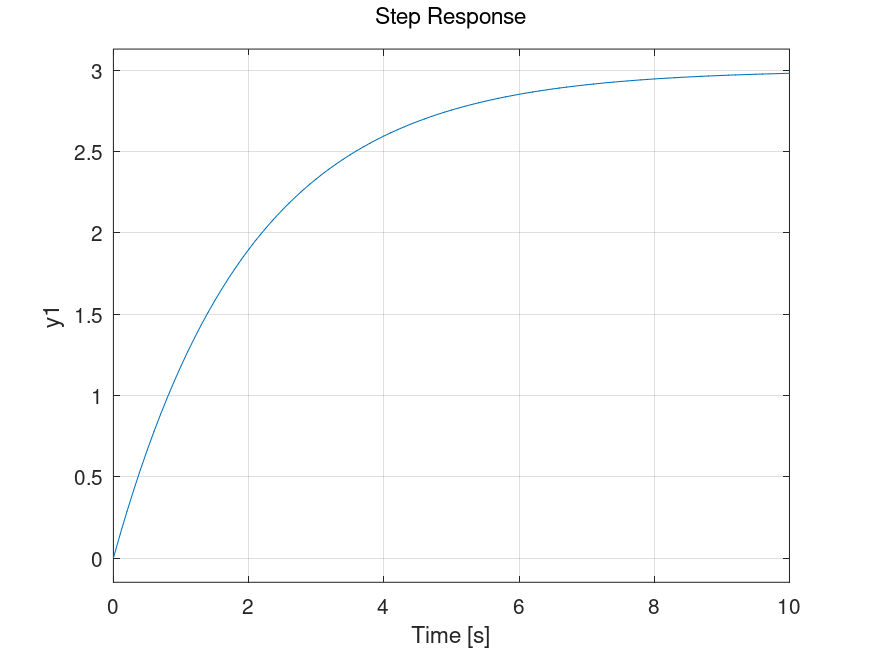
\includegraphics[scale=0.4]{../fig/fig1a.png}
        \caption{Resposta ao degrau \texttt{1a}}
        \label{fig1a}
    \end{figure}
    \begin{figure}[h]
        \centering
        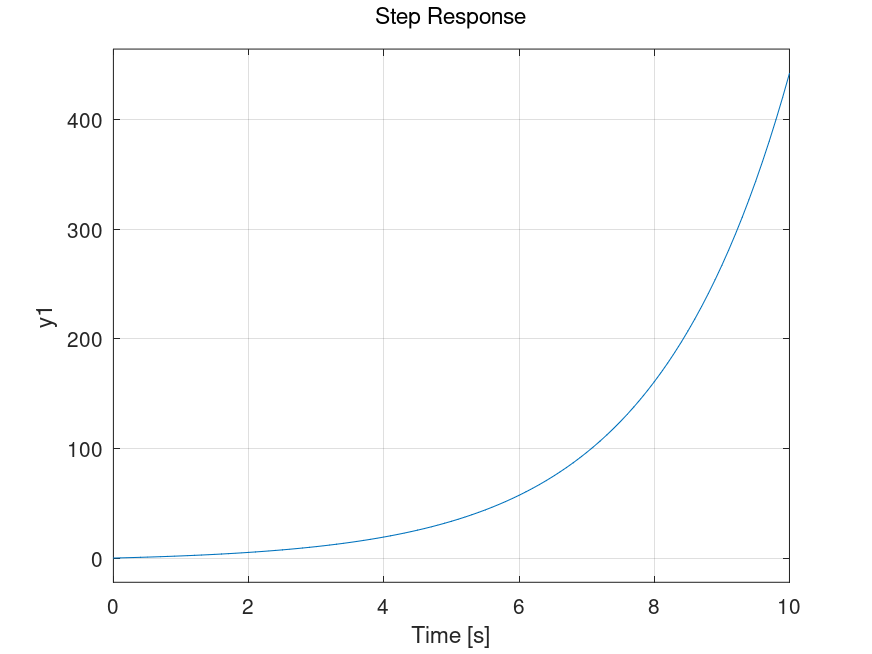
\includegraphics[scale=0.4]{../fig/fig1b.png}
        \caption{Resposta ao degrau \texttt{1b}}
        \label{fig1b}
    \end{figure}
    \begin{figure}[h]
        \centering
        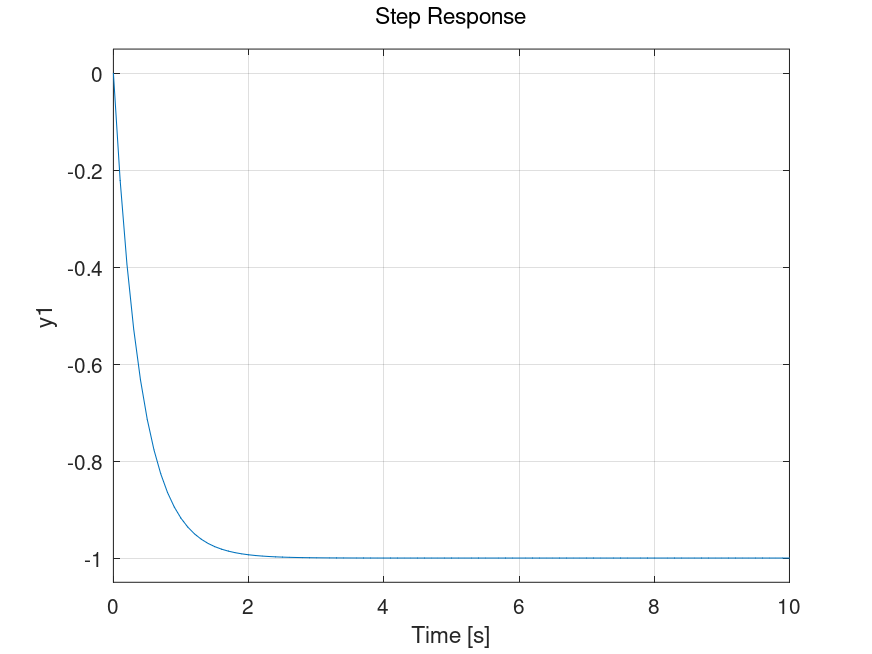
\includegraphics[scale=0.4]{../fig/fig1c.png}
        \caption{Resposta ao degrau \texttt{1c}}
        \label{fig1c}
    \end{figure}
    \begin{figure}[h]
        \centering
        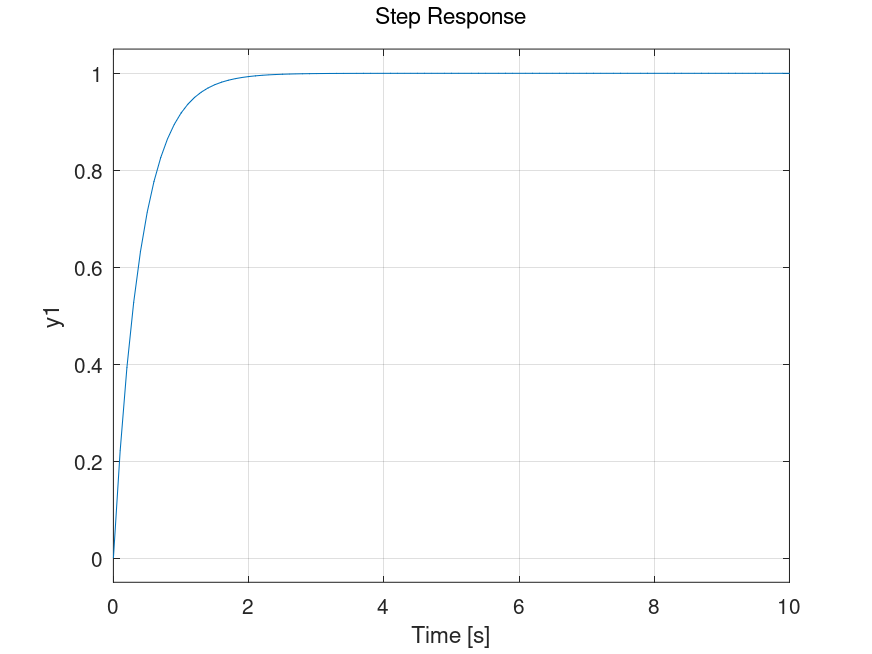
\includegraphics[scale=0.4]{../fig/fig1d.png}
        \caption{Resposta ao degrau \texttt{1d}}
        \label{fig1d}
    \end{figure}
    \begin{figure}[h]
        \centering
        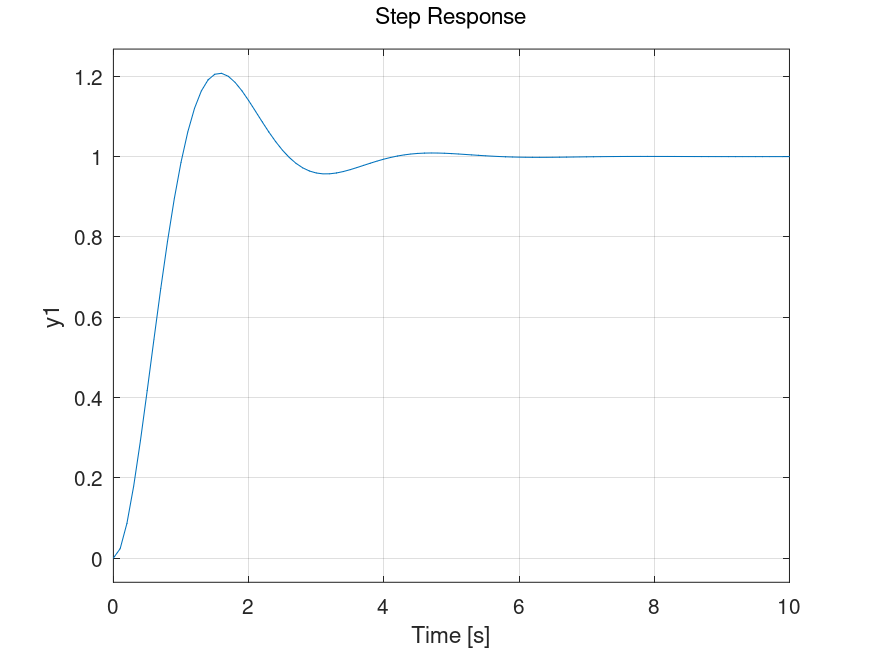
\includegraphics[scale=0.4]{../fig/fig1e.png}
        \caption{Resposta ao degrau \texttt{1e}}
        \label{fig1e}
    \end{figure}
    \begin{figure}[h]
        \centering
        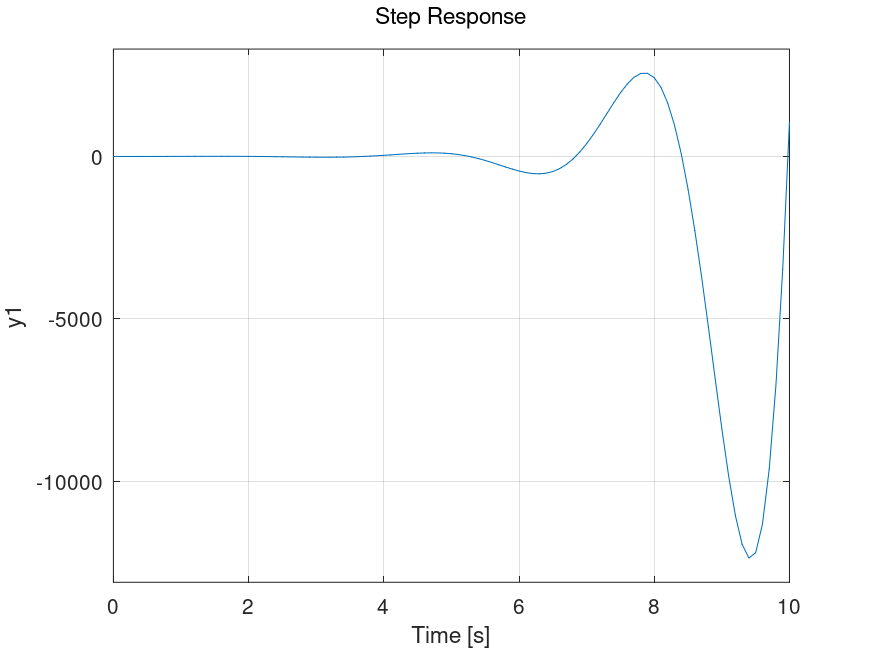
\includegraphics[scale=0.4]{../fig/fig1f.png}
        \caption{Resposta ao degrau \texttt{1f}}
        \label{fig1f}
    \end{figure}
    \begin{figure}[h]
        \centering
        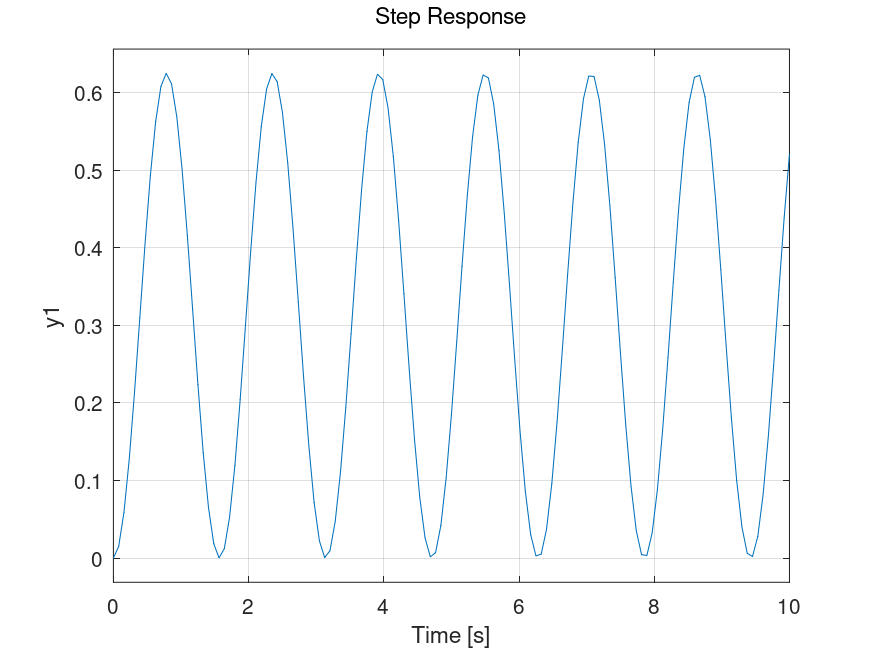
\includegraphics[scale=0.4]{../fig/fig1g.png}
        \caption{Resposta ao degrau \texttt{1g}}
        \label{fig1g}
    \end{figure}
    \begin{figure}[h]
        \centering
        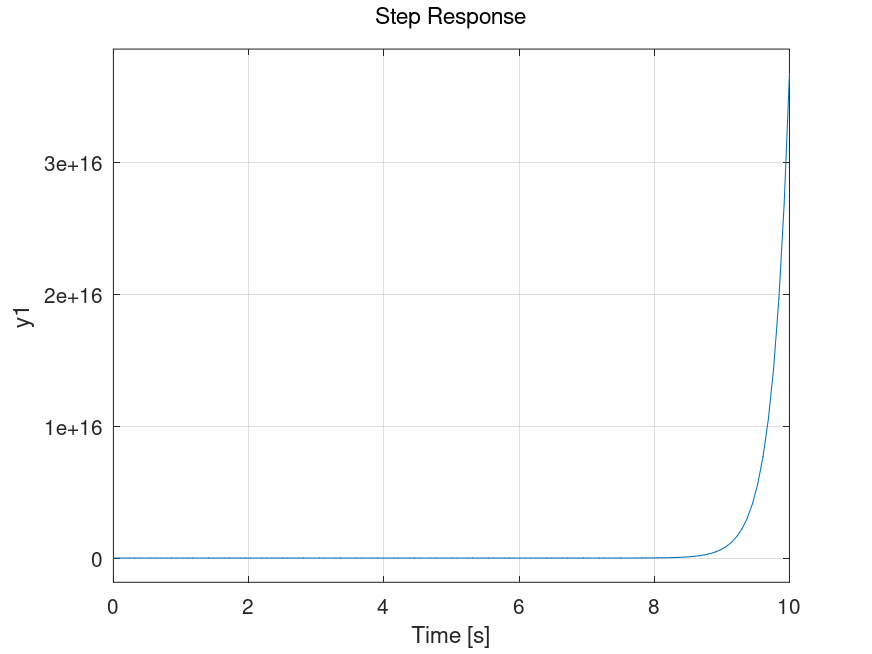
\includegraphics[scale=0.4]{../fig/fig1h.png}
        \caption{Resposta ao degrau \texttt{1h}}
        \label{fig1h}
    \end{figure}
    \begin{figure}[h]
        \centering
        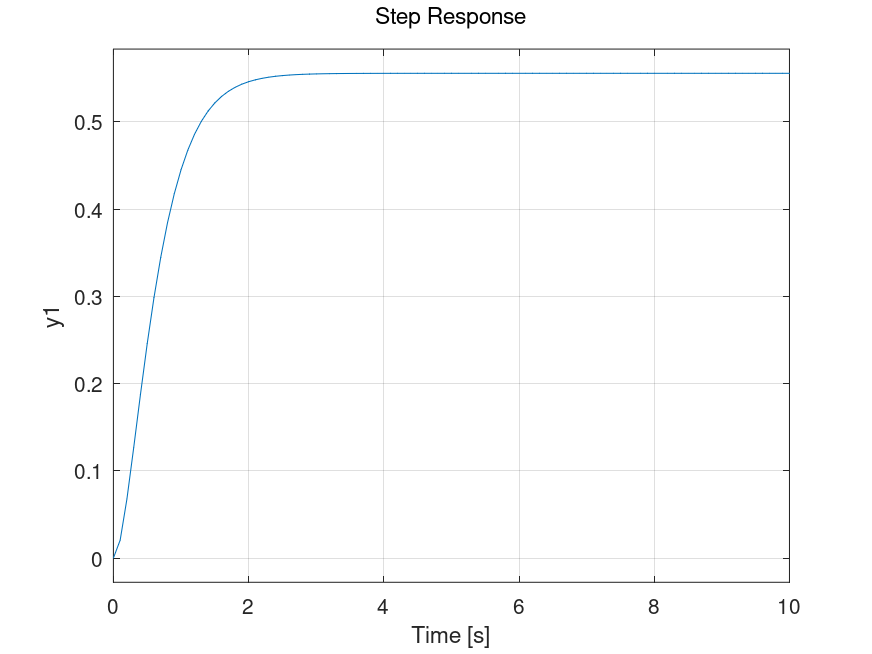
\includegraphics[scale=0.4]{../fig/fig1i.png}
        \caption{Resposta ao degrau \texttt{1i}}
        \label{fig1i}
    \end{figure}
    \begin{figure}[h]
        \centering
        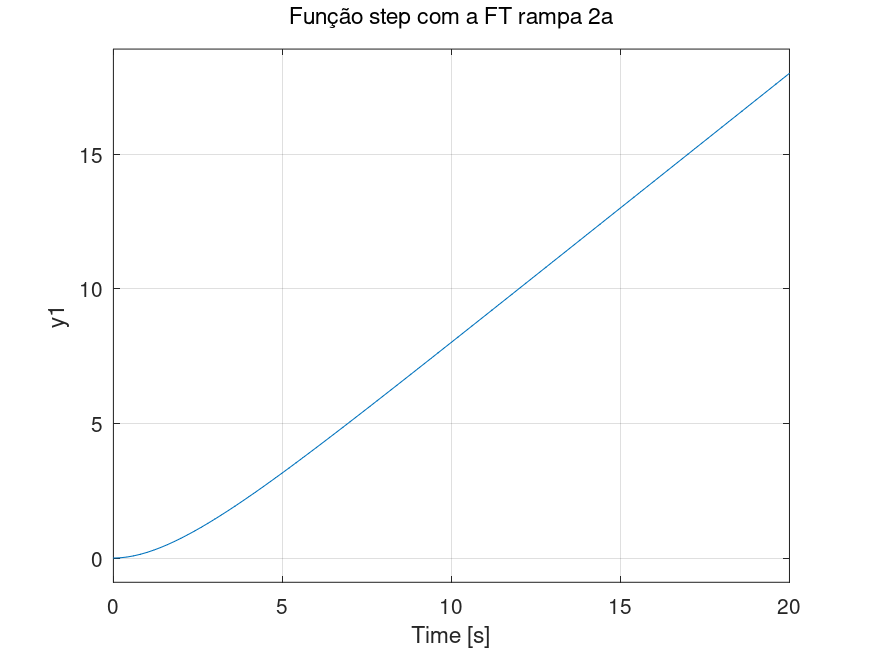
\includegraphics[scale=0.4]{../fig/fig2aStep.png}
        \caption{Resposta com função \texttt{Step} à FT}
        \label{fig2aStep}
    \end{figure}
    \begin{figure}[h]
        \centering
        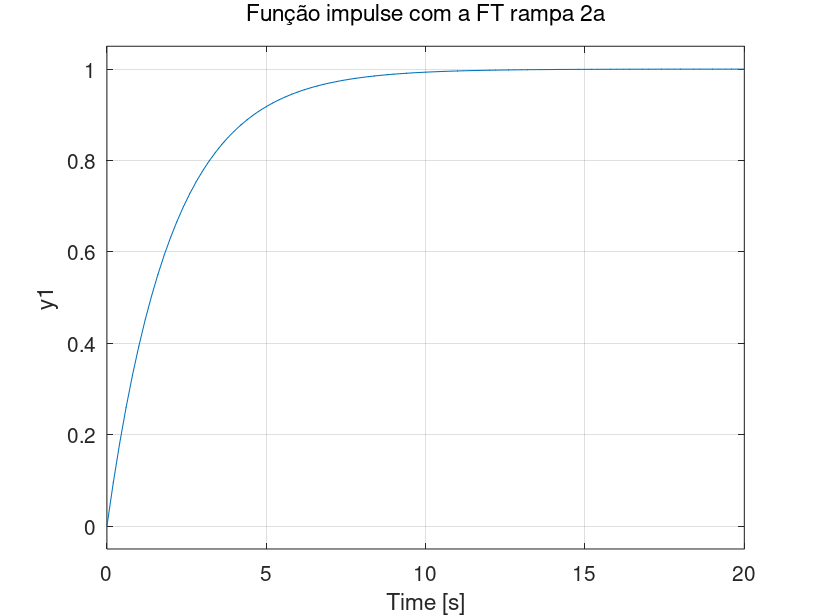
\includegraphics[scale=0.4]{../fig/fig2aImpulse.png}
        \caption{Resposta com função \texttt{Impulse} à FT}
        \label{fig2aImpulse}
    \end{figure}
    \begin{figure}[h]
        \centering
        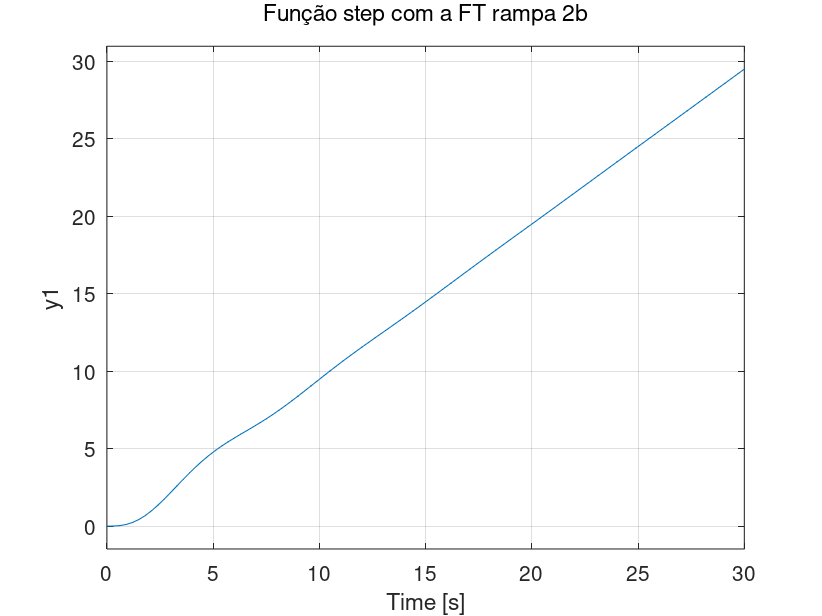
\includegraphics[scale=0.4]{../fig/fig2bStep.png}
        \caption{Resposta com função \texttt{Step} à FT}
        \label{fig2bStep}
    \end{figure}
    \begin{figure}[h]
        \centering
        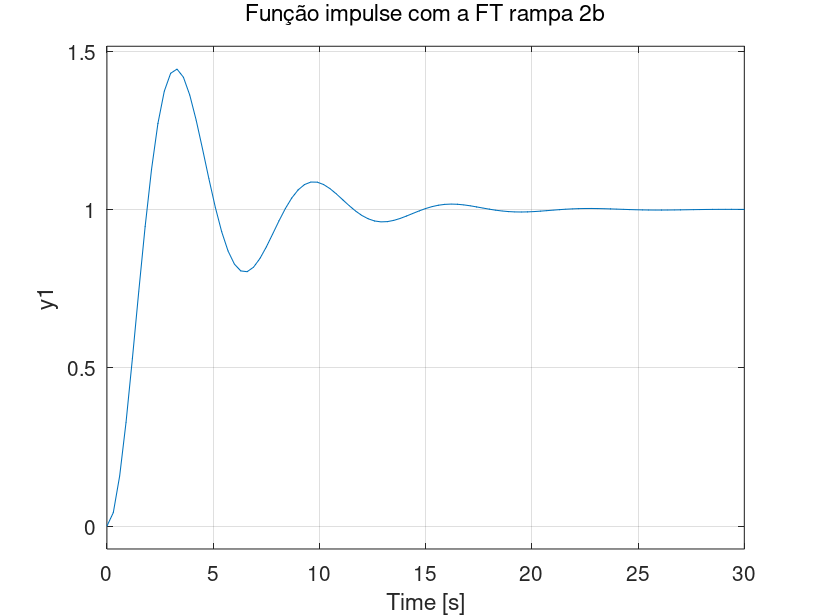
\includegraphics[scale=0.4]{../fig/fig2bImpulse.png}
        \caption{Resposta com função \texttt{Impulse} à FT}
        \label{fig2bImpulse}
    \end{figure}

%%%%%%%%%%%%%%%%%%%%%%%%%%%%%%%%%%%%%%%%%%%%%%%%
% Referências e Bibliografia
%%%%%%%%%%%%%%%%%%%%%%%%%%%%%%%%%%%%%%%%%%%%%%%%

    \clearpage
    \printbibliography

\end{document}
